\subsection{Naboløsninger}

Til den senere anvendelse af simplex metoden anvendes også \textbf{naboløsninger}, som er defineret i Definition \ref{def:nabo}. Undersøgelsen af naboløsninger i simplex metoden som en metode til at reducere antallet af basisløsninger, som skal undersøges når den optimale løsning findes. %Bør omformuleres, er kringlet. Ved ikke: Er det realt det der sker? Ved ikke: Skal SimpLeX staves med stort? Jeg tror da det er det der sker. og simplex er med lille. hermed rettet.

\begin{defn}[Naboløsninger]
	To basisløsninger i $\mathds{R}^n$ siges af være \textbf{naboløsninger}, hvis de deler præcis $n-1$ aktive lineært uafhængige bibetingelser.
	\label{def:nabo}
\end{defn}

Et eksempel på naboløsninger ses i Eksempel \ref{eks:nabo}.

\begin{eks}[Naboløsninger]
De to basisløsninger $\vec{p}=\rvect{4 & 4}^T$ og $\vec{q}=\rvect{10 & 2}^T$ set på Figur \ref{fig:nabo} er naboløsninger, da de har $n-1$ fælles aktive betingelser, hvilket for dette eksempel er $1$ betingelse, nemlig betingelse (2). Basisløsningen $\vec{p}$ har (1) og (2) som aktive betingelser, mens $\vec{q}$ har (2) og (3) som aktive betingelser. %ved ikke, om nemlig bør slettes.
	
	\begin{center}
	\begin{tabular}{l	>{$}r<{$}	>{$}r<{$}	>{$}l<{$} r}
	Maksimer 		& 		4x_1	&	+3 x_2	& \\
	med hensyn til 	&  \ \ 	-2 x_1	& 	+4 x_2	& \leq 8 	& \quad (1)\\
					&  		x_1		& 	+3 x_2	& \leq 16	& \quad (2)\\
					&  \ \ 	x_1		& 			& \leq 10	& \quad (3)\\
	og $x_1 \geq 0$ (4), $x_2\geq 0$ (5).
	\end{tabular}
	\end{center}
	
	\begin{center}
	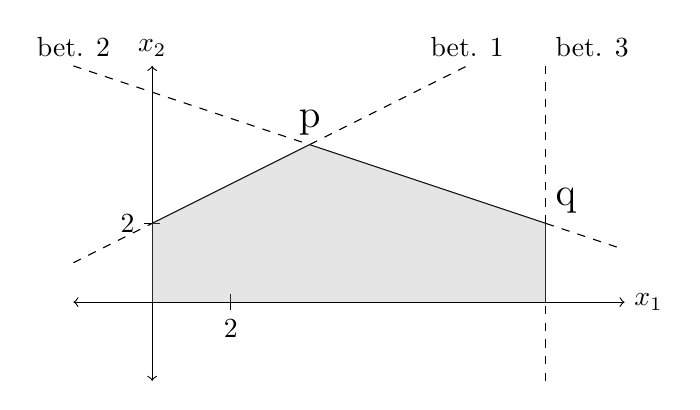
\begin{tikzpicture}
  %laver Grid. godt til når koordinater skal redigeres
  	%\draw[thin,gray!40] (-3,-1) grid (6,3); 
  %x-aksen
  	\draw[<->] (-1,0)--(6,0) node[right]{$x_1$};
  	%\draw[->,red] (2.5,0) -- (2.5,0.5);
  %y-aksen
  	\draw[<->] (0,-1)--(0,3) node[above]{$x_2$};
  	%\draw[->,red] (0,0.5) -- (0.5,0.5);
  	
  %akse-markeringer
  	%\node[left] (xakse) at (0,1) {2};
  	\draw[] (-0.1,1) -- (0.1,1) node[pos=0,left] {2};
  	\draw[] (1,-0.1) -- (1,0.1) node[pos=0,below] {2};
  	
  %ligning 1
	\draw[domain=-1:0,variable=\x,dashed] 	plot({\x},{0.5*\x+1});
	\draw[domain=0:2,variable=\x] 			plot({\x},{0.5*\x+1});
	\draw[domain=2:4,variable=\x,dashed] 	plot({\x},{0.5*\x+1}) node[above] {bet. 1};
  	%\draw[->,red] (1,1.5) -- (1.224,1.05);
	
  %ligning 2
  	\draw[domain=-1:2,variable=\x,dashed] 	plot({\x},{-(1/3)*\x+8/3}) node[above] at (-1,3) {bet. 2} ;
	\draw[domain=2:5,variable=\x] 			plot({\x},{-(1/3)*\x+8/3});
	\draw[domain=5:6,variable=\x,dashed] 	plot({\x},{-(1/3)*\x+8/3});
	%\draw[->,red] (3.5,1.5) -- (3.34,1.026);

  %ligning 3
  	\draw[domain=-1:0,variable=\y,dashed] 	plot({5},{\y});
	\draw[domain=0:1,variable=\y] 			plot({5},{\y});
	\draw[domain=1:3,variable=\y,dashed] 	plot({5},{\y}) node[above right] {bet. 3};
	%\draw[->,red] (5,0.5) -- (4.5,0.5);

  %nodes med navne på punkter
	\node[above] (p) at (2,2) {\Large p};
	\node[above right] (q) at (5,1) {\Large q};

  %løsningsmængden skraveret
	\fill[gray!80,nearly transparent] (0,0) -- (0,1) -- (2,2) -- (5,1) --(5,0) --  cycle;
\end{tikzpicture}
	\captionof{figure}{Løsningsmængde med naboløsninger $p$ og $q$.}
	\label{fig:nabo}
	\end{center}
	
\label{eks:nabo}
\end{eks}

%ved ikke: Må et afsnit slutte med et eksempel?